\section{Data Used}
\subsection{Initial Data}
%The initial architecture has been developed using a data package from LANL for a two-crack system. Data for 250 time steps was provided, with failure occurring at step 52. While useful for testing purposes, this mesh was much coarser than those of the true systems. Hence, for training the network, we used more representative systems of standard HOSS output.

Our preliminary investigation was localized to one LAMMPS simulation run. The data used contained information on bonds, atoms and rings, under the fully periodic condition. 

For simplicity's sake, only the first time step was used to create the basic graph representation in Python. For this analysis, the key data files utilized were the bond information file, used to create the edges between nodes and the post-processed nucleation file which stores information regarding volume and displacement per individual atom.  

\subsection{Training Data}
At the moment, data from one fully periodic simulation is used to train the base case model presented below.  Ultimately, we plan to generalize across different numbers of simulation to create a more sophisticated model and improve predicting accuracy. 

The features we use include cell volume, number of bonds and maximum ring size at initial time step. The label is the dummy indicator of whether or not a certain atom has ever been part of a 20-sized ring during the whole time steps.

\section{Graph Representation}

\subsection{Creation}The first milestone was to implement the basic graph representation in Python. Using the NetworkX library we were able to reconstruct the simulation in Python where a node is an individual atom, Si or O, and an edge is a bond between atoms. With this graph we were able to not only visualize our simulation in a more local window but we are able to create our topological features.

One of our global topological features has shown to be of particular interest, Eigenvector centrality. Using only the information provided during t=0 the eigenvector centrality of our graph appears to be near where the fracture appears at a much later time after nucleation. Figures 3.1 and 3.2 shows this proximity. 

Figure 3.1 shows the eigenvalue centrality of the simulation at t=0. This visual is color coded in a way where blue represents no influence on the network, and the closer the color gets to red indicates the range of influence. With red being the most influential atoms in the simulation. 

Figure 3.2 represents the simulation at t=646,  where the fracture has already nucleated and propagated after some time. Comparing the two visuals one can easily see that there is a close proximity between nucleation and eigenvector centrality. 

While this is only a visual representation there certainly seems to be some indication that eigenvector centrality plays an import role in the nucleation of the simulation. This result will help guide us in our future research and we hope to have a more numerical measurement of this proximity so we can use this global topological feature in our machine learning methods. 

\begin{figure}[H]
    \centering
    \noindent
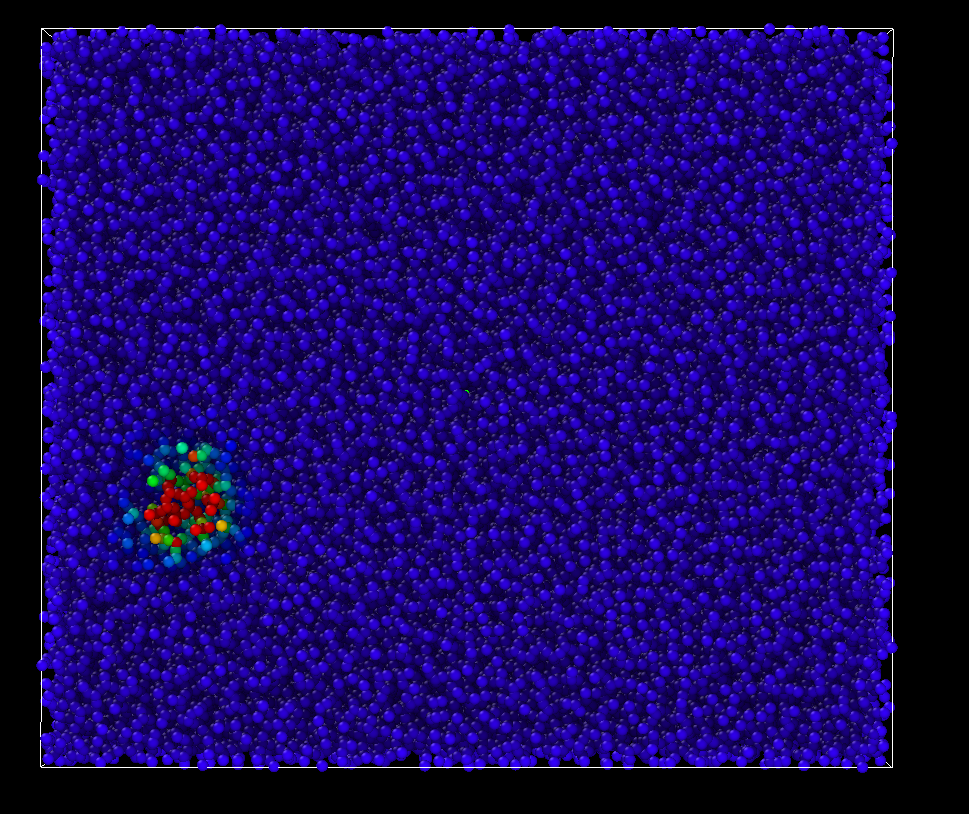
\includegraphics[width=10cm , height = 8cm]{images/left.PNG}
    \caption{Eigenvector Centrality at time step 0}
    \label{fig:eig_cent}


    \centering
    \noindent
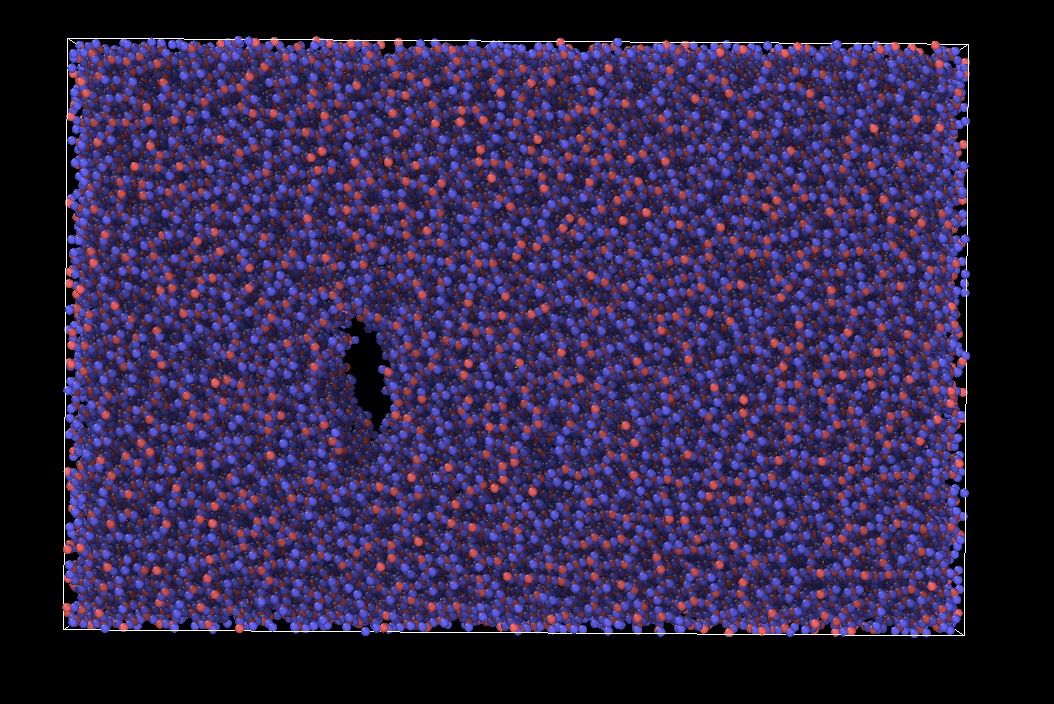
\includegraphics[width=12cm , height = 8cm]{images/right.PNG}
    \caption{Simulation at time step 646}
    \label{fig:right}
\end{figure}

\subsection{Feature Correlations}
After the graph had been created are now able to take a look at how the features of the atoms play a role within the structure and how they correlate with other quantities of interest within the system. One such structure is the role bridging oxygen play within the global structure of the simulation. 

Below in Figure 3.3 we can see how well specific feature correlate with each other. On this specific heat map we have both degree and eigenvector centrality measures. As you can see degree centrality is perfectly correlated with the number of bridging oxygen one away. Whereas, volume at t = 0 appears to have a negative correlation on the number of bridging oxygen 1 away and a minor correlation ~10 percent on the number of bridging oxygen 2 away. 

While we have no found any major correlation between features the graph representation we have created has allowed us the freedom of investigation, and any future features can be measured by their correlation on the simulation. 


\begin{figure}[H]
    \centering
    \noindent
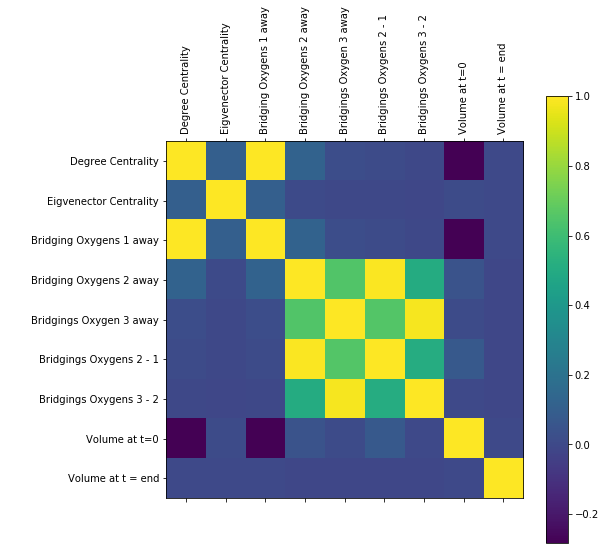
\includegraphics[width=10cm , height = 9cm]{images/Heatmap.PNG}
    \caption{Heat map of Pearson correlation coefficients.}
    \label{fig:heatmap}
\end{figure}

\section{Results}
In this section, we presents the preliminary results we obtained from base case toy models, which are Logistic Regression and Support Vector Machine with imbalanced class.

{\color{red} For the methods below: What features are you using?  What labels are you trying to predict?  Provide all details needed for someone to reproduce your work.}

\subsection{Logistic Regression}
Logistic Regression is a static model that we use to predict the labels with probabilities of the underlying classes. However, due to imbalanced class, the model ignores the false negatives and predicts all the labels to be negative to obtain a high accuracy. 

\subsection{SVM with imbalanced class}

To tackle the problem of imbalanced class, we also implemented a basic Support Vector Machine model with a penalty on the imbalanced classes. The model obtains an accuracy of 66\% and an area under the AUROC curve of 0.58 as presented by figure \ref{fig:svm_roc}.

\begin{figure}[H]
    \centering
    \noindent
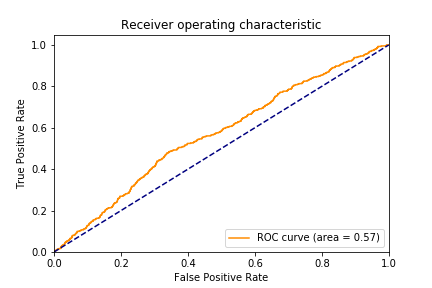
\includegraphics[width=8cm , height = 6cm]{images/svm_roc.png}
    \caption{Plot of False Positive Rate against True Positive Rate for Support Vector Machine Model}
    \label{fig:svm_roc}
\end{figure}

\iffalse
\subsection{Crack Identification}
In converting HOSS FDEM output to graph form, recall that we follow two rules to preserve the integrity of the fracture network:
\begin{itemize}
	\item Edge crack identification must remain fixed over time.
 	\item Crack identity must be preserved through coalescence.
\end{itemize} 
By preserving the identification of each crack through both time and coalescence, we provide the necessary index for identification and tracking of each crack across all time steps, as well as correct attribution of feature metrics to the appropriate locations.
          
\subsection{Graph Data Matrices}
In order to set up the Graph Convolutional Neural Network architecture, we need to define the metrics used in the Adjacency and Feature matrices.\\
Distance Metrics:
        \begin{itemize}
        \item Coalescence (binary)
        \item Tip Intersect Distance  
        \item Shortest Euclidean Distance
        \item Minimum Damage Path
        \end{itemize}       
Features:
    \begin{itemize}
	\item Maximal horizontal projected crack tip Euclidean length
	\item Maximal vertical projected crack tip Euclidean length 
	\item Crack extreme tip Euclidean length
    \item Maximal Crack path Euclidean length between two tips
    \item Total path length including all crack tips
    \item Total crack damage
    \item Max tip stress
    \item Mean tip stress
	\end{itemize}
    
Functions were created to calculate and extract this data from HOSS simulation data to create graph data matrices for each HOSS time step.  

\section{R-GCN Setup}
The second milestone is to construct a working algorithm and model from the graph representation to predict the behavior of the fracture network over time. We accomplish this by using the Keras library for Python as a basis for building our RNN \cite{chollet2015keras}. The model simultaneously outputs predictions for both the features and each distance metric while following precisely the architecture presented in section 3.4. The implementation of the graph convolutional layer is taken from \cite{kipf2016semi}.

\section{Results}

As mentioned, our preliminary results come from training on three twenty-crack systems. In order to augment training data and increase the generalization ability of the network, we randomly take slices of 25 time steps. This allows for the network to learn from varying starting points and works to prevent overfitting. Also, the features are normalized across feature type before training using a normalizing matrix. Given that some features, such as total crack damage, can become large near the end of the system this serves to condense values to a far smaller range and enable better learning. Ultimately, the feature predictions can be transformed back to their original scale through the same normalizing matrix from the training data.

Our goal is for our network to be able to generalize, to predict systems on which it has not been trained. However, for these initial tests, we perform the more simple task of predicting the evolution of one of the three crack systems from time step 0 to the final time step. As described in the methods section, there will first be a prediction for time step 1 given input at time step 0, then for time step 2 given input at time steps 0 and predicted output from time step 1 and so on. This will test the general ability of the architecture to learn and find patterns.

\begin{figure}[!htb]
\centering
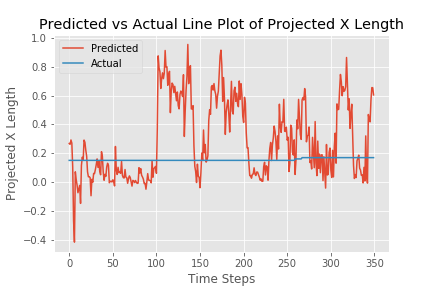
\includegraphics[width=0.8\textwidth]{images/Projected_X_Length_compare_transformed}
\caption{Plot comparing the predicted values against true values for projected $x$ length of crack 19.}
\label{fig:proj_y}
\end{figure}

\begin{figure}[!htb]
\centering
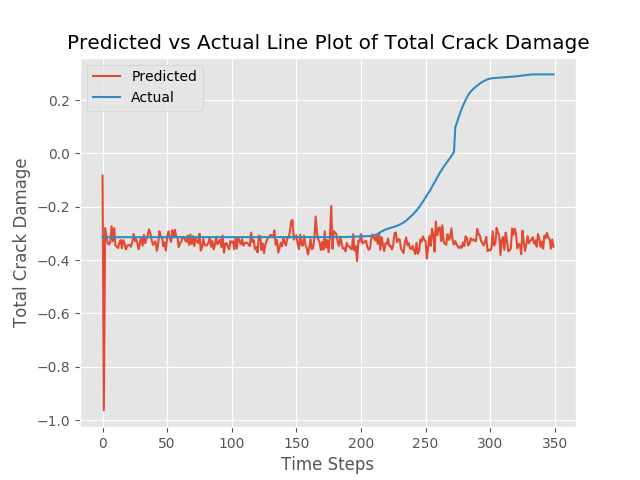
\includegraphics[width=0.8\textwidth]{images/Total_Crack_Damage_compare}
\caption{Plot comparing the normalized predicted values against the normalized true values for total crack damage in crack 4.}
\label{fig:tot_dam}
\end{figure}

In figures \ref{fig:proj_y} and \ref{fig:tot_dam}, selected results for feature prediction are presented. In figure \ref{fig:proj_y},we plot the projected $x$ length vs.\ time, for a simulated system with total size of 3 in the $x$ direction and 2 and in the $y$ direction.
%The spatial scale of the material in this simulation run is 3 by 2( Total X length 3, Y length 2).
The actual projected $x$ length does not change until time step 200.  Many of the features in a given simulation are essentially constant, and thus in our limited training, the model has overfit to these examples. This is illustrated in figure \ref{fig:tot_dam}, where the damage changes near the end of the simulation, yet our network is unable to predict the change.

As the output from HOSS is not deterministic, the comparison between distributions of crack features is more meaningful than feature comparisons on specific cracks. In figure \ref{fig:mean_proj_x_length}, we plot our prediction for the mean projected $x$ length of all cracks, along with the actual mean projected $x$ length. The band represents plus and minus one standard deviation of the crack features. As we can see, the mean and variance in our prediction is tracking the actual when the cracks start growing quickly around time step 220.

Ultimately, these preliminary results showed us that the network has the ability to learn. It does not predict each feature perfectly, yet it does give meaningful predictions for distributions over all cracks in the system. These results leave us optimistic for future results given additional network refinement and more substantial training.

\begin{figure}[!htb]
\centering
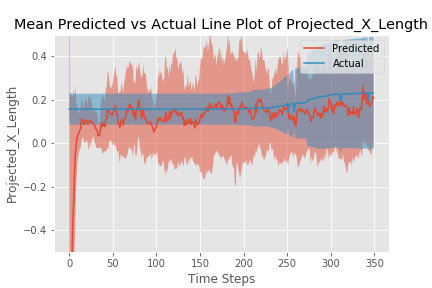
\includegraphics[width=0.8\textwidth]{images/Projected_X_Length_mean_variance_compare_ylim_test}
\caption{Plot comparing the mean predicted values against mean true values for projected $x$ length of all cracks. Shaded bands show one standard deviation above and below mean.}
\label{fig:mean_proj_x_length}
\end{figure}


\fi